\documentclass[a4paper,12pt,oneside]{book}
\usepackage[T1]{fontenc}                                      
\usepackage[utf8]{inputenc}                               
\usepackage[italian]{babel}
\usepackage{amsfonts}
\usepackage{amsthm}
\usepackage{amsmath,amssymb}
\usepackage{array}
\usepackage{arydshln}
\usepackage{braket}
\usepackage{blindtext}
\usepackage{calc}
\usepackage{cancel}
\usepackage{caption}
\usepackage{epsfig}
\usepackage{eucal}
\usepackage{fancyhdr}
\usepackage{geometry}
\usepackage{graphicx}
\usepackage{indentfirst}
\usepackage{hhline}
\usepackage{hyperref}
\hypersetup{
			colorlinks=true,
			linkcolor=black,
			anchorcolor=black,
			citecolor=black,
			urlcolor=black,
			pdftitle={Appunti di Meccanica Quantistica},
			pdfauthor={Vittorio Lubicz}
}

\usepackage{latexsym}
\usepackage{listings} 
\usepackage{longtable}
\usepackage{makeidx}
\usepackage{mathrsfs}
\usepackage{mathdots}
\usepackage{multirow}
\usepackage{nicefrac}
\usepackage{pdfpages}
\usepackage{physics}
\usepackage{setspace}
\usepackage{tikz}
\usepackage{tikz-3dplot}
\usepackage{textcomp}
\usepackage{titlesec,color}
\usepackage{vmargin}
\setpapersize{A4}
\setmarginsrb{35mm}{30mm}{35mm}{30mm}%
             {0mm}{10mm}{0mm}{10mm}



\definecolor{gray75}{gray}{0.75}
\newcommand{\hsp}{\hspace{20pt}}

\titleformat{\chapter}[hang]{\huge\bfseries}{\myfont{\textit{\large{\chaptername\hspace{1pt} \thechapter\hspace{3pt}}}}\textcolor{gray75}{$\mid$}\hspace{0.4cm}}{0pt}{\myfont{\huge\bfseries}}

\titleformat{\section}[hang]{\large\bfseries}{\myfont{\textit{\normalsize{\thesection\hspace{2pt}}}}\hspace{0.4cm}}{0pt}{\myfont{\Huge\bfseries}}

\titleformat{\subsection}[hang]{\large\bfseries}{\myfont{\textit{\small{\thesubsection\hspace{2pt}}}}\hspace{0.4cm}}{0pt}{\myfont{\huge\bfseries}}

\renewcommand{\chaptermark}[1]{\markboth{#1}{}}
\renewcommand{\sectionmark}[1]{\markright{#1}}
\newcommand*{\myfont}{\fontfamily{ppl}\selectfont}

\begin{document}

%*****************LAYOUT PAGINE**************************
\fancypagestyle{plain}{%
\fancyhf{} % cancella tutti i campi di  intestazione e pi\`e di pagina
\fancyfoot[C]{\bfseries \myfont{\thepage}} % tranne il centro
\renewcommand{\headrulewidth}{0pt}
\renewcommand{\footrulewidth}{0pt}}

\fancypagestyle{VS}{
\headheight = 15pt
\lhead[\myfont{\textit{\textbf{\thechapter\nouppercase{\leftmark}}}}]{\myfont{\textit{\textbf{\nouppercase{\leftmark}}}}}
\chead[]{}
\rhead[\myfont{\textbf{\thepage}}]{\myfont{\textbf{\thepage}}}

\lfoot[]{}
\cfoot[]{}
\rfoot[]{}
}
%*******************************************************



\pagestyle{VS}
\setcounter{chapter}{15}
\setcounter{page}{164}
\chapter{Momento angolare}
\section[Rotazioni, momento angolare e regole di commutazione]{Rotazioni, momento angolare e regole di commutazione per gli operatori momento angolare\footnote{S3.1; LL26}}
Nella meccanica quantistica, così come nella meccanica classica, \textbf{il momento angolare è il generatore delle rotazioni infinitesime}.\\
Se indichiamo con $D_{\widehat{n}} (d\varphi)$ l'operatore unitario che induce una rotazione di un angolo infinitesimo $d\varphi$ attorno all'asse caratterizzato dal vettore $\widehat{n}$ abbiamo allora
\begin{equation}
D_{\widehat{n}} (d\varphi)=1-\frac{i}{\hbar}\vec{J}\cdot \widehat{n}\ d\varphi ,
\end{equation}
dove $\vec{J}$ è \textbf{l'operatore momento angolare}. Questa equazione può essere considerata la \textbf{definizione} nella meccanica quantistica dell'operatore momento angolare.\\
Una rotazione finita si può ottenere associando successivamente rotazioni infinitesime attorno allo stesso asse. Così ade esempio, per una rotazione finita di un angolo $\phi$ attorno all'asse $z$, otteniamo
\begin{eqnarray}
D_z (\phi) &=& \lim _{N\rightarrow \infty} \left(1-\frac{i}{\hbar} J_z \frac{\phi}{N}\right) ^N= \nonumber \\
&=& \lim _{N\rightarrow \infty} e^{N\log\left(1-\frac{i}{\hbar} J_z \frac{\phi}{N}\right)}= \lim _{N\rightarrow \infty} e^{N\left(-\frac{i}{\hbar} J_z \ \frac{\phi}{N}\right)},
\end{eqnarray}
ossia
\begin{equation}
D_z (\phi)=e^{-\frac{i}{\hbar} J_z \phi}.
\end{equation}
\textbf{L'avere assunto che il momento angolare è il generatore delle rotazioni spaziali implica che, per un sistema invariante rispetto a rotazioni attorno a un determinato asse, si conserva la componete del momento angolare lungo quell'asse.}\\
In particolare poi, le proprietà di isotropia dello spazio (ossia l'equivalenza di tutte le direzioni nello spazio) implica che l'hamiltoniano di un sistema isolato deve essere invariante rispetto a rotazioni di un angolo arbitrario attorno a un asse qualsiasi. \textbf{La legge di conservazione del momento angolare di un sistema isolato è dunque conseguenza della proprietà di isotropia dello spazio}.\\

È una proprietà ben nota delle rotazioni il fatto che \textbf{rotazioni attorno ad uno stesso asse commutano, mentre rotazioni attorno ad assi diversi non commutano}. Così ad esempio una rotazione di $\pi /2$ attorno all'asse $z$ seguita da una rotazione di $\pi /2$ attorno all'asse $x$ produce un risultato diverso di quello ottenuto con una rotazione di $\pi /2$ attorno all'asse $x$ seguita da una rotazione di $\pi /2$ attorno all'asse $z$:\\
\begin{figure}[!htbp]
\begin{center}
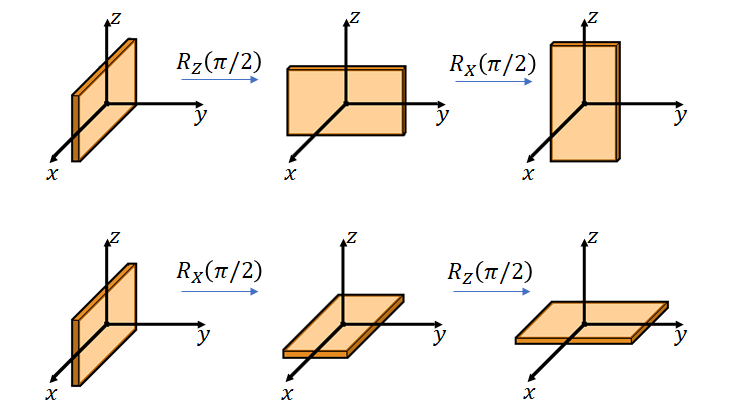
\includegraphics[width=10cm]{immagini/cap_16/fig_16_1.png}
\end{center}
\end{figure}


In termini dell'azione degli operatori di rotazione du un generico vettore di stato $\vert \alpha \rangle$ questo implica
\begin{equation}
D_x (\pi/2) D_z (\pi/2) \vert \alpha \rangle \neq D_x (\pi/2) D_x (\pi/2) \vert \alpha \rangle ,
\end{equation}
o, equivalentemente, per l'arbitrarietà dello stato $\vert \alpha \rangle$,
\begin{equation}
[D_x (\pi/2); D_z (\pi/2)] \neq 0 .
\end{equation}
Per stabilire quantitativamente le regole di commutazione degli operatori di rotazione attorno ad assi diversi, dobbiamo considerare con maggior dettaglio le proprietà di commutazione delle rotazioni.\\
A tale scopo ricordiamo che a ciascuna rotazione, diciamo di un angolo $\varphi$ attorno ad un asse definito dal versore $\widehat{n}$, può essere associata una \textbf{matrice ortogonale} $R_{\widehat{n}} (\varphi)$. Il significato di questa matrice è che un vettore $\vec{v}$ di componenti $(v_x, v_y v_z) $ ( che può rappresentare ad esempio la posizione di una particella nello spazio), viene trasformato, a seguito della rotazione nel vettore $\vec{v'}$ legato a $\vec{v}$ dalla relazione
\begin{equation}
\vec{v'}= R_{\widehat{n}} (\varphi)\vec{v}.
\end{equation}
L'ortogonalità della matrice $R$ segue dal fatto che le rotazioni lasciano invariati i moduli dei vettori:
\begin{equation}
\vec{v'}\cdot\vec{v} = \vec{v}R^T R \vec{v}= \vec{v}\cdot\vec{v} \qquad \Rightarrow \quad
 R^T R =1.
\end{equation}
È semplice derivare l'espressione della matrice di rotazione associata ad esempio ad una rotazione di un angolo $d\varphi $ attorno all'asse $z$. Esprimendo le componenti del vettore $\vec{v}$ in coordinate polari,
\begin{equation}
\begin{cases}
v_x = v \sin\theta \cos \varphi ,\\
v_y = v \sin\theta \sin \varphi ,\\
v_z = v \cos\theta ,
\end{cases}
\end{equation}
si ha che il vettore $\vec{v}$ si trasforma, per effetto della rotazione, nel vettore $\vec{v'}$ di componenti:
\begin{equation}
\begin{cases}
v'_x = v \sin\theta \cos (\varphi +d\varphi )= v_x \cos d\varphi - v_y \sin d\varphi ,\\
v'_y = v \sin\theta \sin (\varphi +d\varphi ) = v_x \sin d\varphi + v_y \cos d\varphi ,\\
v'_z = v \cos\theta = v_z .
\end{cases}
\end{equation}
La matrice $R_z (d\varphi)$ ha dunque la forma
\begin{equation}
R_z (d\varphi)=
\begin{pmatrix}
\cos d\varphi & -\sin d\varphi & 0\\
\sin d\varphi & \cos d\varphi & 0 \\
0 & 0 & 1 \\
\end{pmatrix}
\end{equation}
Per studiare le proprietà di commutazione delle rotazioni è conveniente considerare rotazioni infinitesime. Ponendo $\varepsilon =d\varphi$ e sviluppando la precedente matrice fino al secondo ordine in $\varepsilon$ troviamo:
\begin{equation}
R_z (\varepsilon)=
\begin{pmatrix}
1-\varepsilon ^2 /2 & -\varepsilon & 0\\
\varepsilon & 1-\varepsilon ^2/2 & 0 \\
0 & 0 & 1 \\
\end{pmatrix}
+ O(\varepsilon ^3).
\end{equation}
Le corrispondenti matrici si rotazione attorno agli assi $x$ e $y$ si possono ottenere con permutazioni cicliche di $x$, $y$ e $z$:
\begin{equation}
x\rightarrow y,\ y\rightarrow z,\ z\rightarrow x,
\end{equation}
si ottiene in tal modo:
\begin{equation}
R_x (\varepsilon)=
\begin{pmatrix}
1 & 0 & 0\\
0 & 1-\varepsilon ^2/2 & -\varepsilon \\
0 & \varepsilon & 1-\varepsilon ^2/2 \\
\end{pmatrix}
+ O(\varepsilon ^3),
\end{equation}
\begin{equation}
R_y (\varepsilon)=
\begin{pmatrix}
1-\varepsilon ^2/2 & 0 & \varepsilon\\
0 & 1 &0 \\
- \varepsilon & 0 & 1-\varepsilon ^2/2 \\
\end{pmatrix}
+ O(\varepsilon ^3).
\end{equation}
Consideriamo ora una rotazione di angolo $\varepsilon$ attorno all'asse $y$ seguita da una rotazione di angolo $\varepsilon$ attorno all'asse $x$. La corrispondente matrice di rotazione è:
\begin{equation}
R_x (\varepsilon)R_y (\varepsilon)=
\begin{pmatrix}
1-\varepsilon ^2/2 & 0 & \varepsilon \\
 \varepsilon ^2 & 1-\varepsilon ^2/2 & -\varepsilon \\
-  \varepsilon & \varepsilon & 1-\varepsilon ^2 \\
\end{pmatrix}
+ O(\varepsilon ^3)
\end{equation}
Se consideriamo invece rotazione di angolo $\varepsilon$ attorno all'asse $x$ seguita da una rotazione di angolo $\varepsilon$ attorno all'asse $y$ otteniamo la matrice di rotazione
\begin{equation}
R_y (\varepsilon)R_x (\varepsilon)=
\begin{pmatrix}
1-\varepsilon ^2/2 & \varepsilon ^2 & \varepsilon \\
 0 & 1-\varepsilon ^2/2 & -\varepsilon \\
-  \varepsilon & \varepsilon & 1-\varepsilon ^2 \\
\end{pmatrix}
+ O(\varepsilon ^3)
\end{equation}
NB $\displaystyle{\left[\left( R_y R_x\right) ^T = R_x ^T R_y ^T=R_xR_y+(\varepsilon\rightarrow -\varepsilon)\right]}$.\\
Dal confronto di questi risultati vediamo che
\begin{equation}
R_x (\varepsilon)R_y (\varepsilon)-R_y (\varepsilon)R_x (\varepsilon)=
\begin{pmatrix}
0 & - \varepsilon ^2 & 0 \\
 \varepsilon ^2 & 0 & 0 \\
0 & 0& 0\\
\end{pmatrix}
= R_z(\varepsilon ^2)-1+ O(\varepsilon ^3),
\end{equation}
che definisce la proprietà di commutazione di due rotazioni successive infinitesime attorno agli assi $x$ ed $y$.\\
La stessa proprietà deve essere soddisfatta dagli operatori che inducono le corrispondenti rotazioni dei vettori di stato in meccanica quantistica, ossia:
\begin{equation}
D_x (\varepsilon)D_y (\varepsilon)-D_y (\varepsilon)D_x (\varepsilon)=D_z(\varepsilon ^2)-1+ O(\varepsilon ^3).
\end{equation}
In termini degli operatori momento angolare, questa relazione implica:
\begin{eqnarray}
& &D_x (\varepsilon)D_y (\varepsilon)-D_y (\varepsilon)D_x (\varepsilon)= \nonumber\\
& & = \left(1-\frac{i\varepsilon}{\hbar} J_x -\frac{\varepsilon ^2}{2\hbar ^2}J_x ^2\right)\left(1-\frac{i\varepsilon}{\hbar} J_y -\frac{\varepsilon ^2}{2\hbar ^2}J_y ^2\right)- \left( x \leftrightarrow y\right) =\nonumber \\
& &= \left(1-\frac{i\varepsilon}{\hbar} J_x-\frac{i\varepsilon}{\hbar} J_y-\frac{\varepsilon ^2}{2\hbar ^2}J_x-\frac{\varepsilon ^2}{2\hbar ^2}J_y-\frac{\varepsilon ^2}{\hbar ^2}J_xJ_y \right) - \left( x \leftrightarrow y\right) = \nonumber \\
& & = -\frac{\varepsilon ^2}{\hbar ^2}\left(J_xJ_y-J_y J_x\right)= \nonumber \\
& & = D_z (\varepsilon ^2)- = \left(1-\frac{i\varepsilon ^2}{\hbar} J_z-\right)=-\frac{i\varepsilon ^2}{\hbar} J_z, 
\end{eqnarray}
ossia
\begin{equation}
[ J_x, J_y ] = i\hbar J_z.
\end{equation}
Utilizzando le permutazioni cicliche di $x$, $y$ e $z$ possiamo derivare le regole di commutazione per le altre componenti del momento angolare:
\begin{equation}
[ J_y, J_z ] = i\hbar J_x,
\end{equation}
\begin{equation}
[ J_z, J_x ] = i\hbar J_y,
\end{equation}
o in forma compatta per due componenti arbitrarie
\begin{equation}
[ J_i, J_j ] = i\hbar \varepsilon _{ikj}J_k.
\label{eq:cap16_1}
\end{equation}
Queste equazioni sono note come le \textbf{relazioni fondamentali di commutazione del momento angolare}.\\
Sottolineiamo come \textbf{queste relazioni di commutazione seguono solamente dall'assunzione che $J_k$ è il generatore della rotazione attorno all'asse k-esimo e dalla proprietà di non commutatività delle rotazioni}.\\
\textbf{Le relazioni di commutazione (\ref{eq:cap16_1}) implicano che, in generale, le tre componenti del momento angolare non possono avere simultaneamente valori determinati}. A questo proposito il momento angolare differisce essenzialmente dall'impulso, le cui tre componenti sono misurabili simultaneamente.		
Con gli operatori $J_x$, $J_y$ e $J_z$ formiamo l'\textbf{operatore} del \textbf{quadrato del momento angolare}:
\begin{equation}
J^2 = J_x ^2 + J_y ^2 + J_z ^2.
\end{equation}
Questo operatore commuta con ciascuno degli operatori $J_x$, $J_y$ e $J_z$:
\begin{equation}
[J^2, J_k]=0. \quad (k=1,2,3)
\label{eq:cap16_2}
\end{equation}
Infatti, considerando ad esempio il caso $k=3$ ed utilizzando le relazioni di commutazione (\ref{eq:cap16_1}) otteniamo:
\begin{eqnarray}
[J^2, J_z] &=& [J_x ^2+J_y^2+J_z ^2, J_z] = [J_x ^2, J_z]+[J_y ^2, J_z]= \nonumber \\
& =& J_x[J_x, J_z]+[J_x, J_z]J_x+J_y[J_y, J_z]+[J_y, J_z]J_y =  \nonumber \\
& = & J_x (-i\hbar J_y)+ (-i\hbar J_y)J_x+ J_y (i\hbar J_x)+(i\hbar J_x)J_y = \nonumber \\
& = & 0.  
\end{eqnarray}
(N.B.: abbiamo usato la proprietà generale dei commutatori\\ $\displaystyle{[AB,C]=A[B,C]+[A,C]B}$).\\
Dal punto di vista fisico, le relazioni (\ref{eq:cap16_2}) significano che \textbf{il quadrato del momento angolare (cioè il suo valore assoluto) può avere valori determinati contemporaneamente con una delle sue componenti}.
\section[Autovalori ed elementi di matrice degli operatori di momento angolare]{Autovalori ed elementi di matrice degli operatori di momento angolare\footnote{S3.5, LL27}}
Consideriamo il problema di determinare gli autovalori e gli autovettori simultanei del quadrato del momento angolare $J^2$ e di una sua componente lungo un determinato asse, diciamo $J_z$. Indichiamo rispettivamente con $a$ e $b$ questi autovalori.\\
Cerchiamo cioè le soluzioni delle equazioni
\begin{eqnarray}
& &J^2 \vert a, b \rangle = a \vert a, b \rangle , \\
& &J_z \vert a, b \rangle = b \vert a, b \rangle .
\end{eqnarray}
A tale scopo risulta conveniente, in luogo degli operatori $J_x$ e $J_y$, introdurre le loro combinazioni complesse
\begin{equation}
J_{\pm} = J_x \pm i J_y .
\end{equation}
Utilizzando le relazioni di commutazione (\ref{eq:cap16_1}) per le componenti del momento angolare possiamo calcolare
\begin{eqnarray}
[J_z , J_{\pm}] & = & [J_z , J_x \pm i J_y] = [J_z , J_x] \pm i [J_z ,J_y] = \nonumber \\
& = & i\hbar J_y \pm i (-i\hbar J_x) = \pm \hbar (J_x \pm i J_y ) = \pm \hbar J_{\pm} .
\end{eqnarray}
Dunque
\begin{equation}
[J_z , J_{\pm}] = \pm \hbar J_{\pm} .
\label{eq:cap16_3}
\end{equation}
Dalle relazioni di commutazione (\ref{eq:cap16_2}) segue anche immediatamente
\begin{equation}
[J^2 , J_{\pm}]=0 .
\label{eq:cap16_4}
\end{equation}
Per determinare il significato fisico degli operatori $J_{\pm}$ esaminiamo l'azione di $J_z$ sugli stati $J_{\pm} \vert a, b \rangle$:
\begin{eqnarray}
J_zJ_{\pm} \vert a, b \rangle & =& \left( [J_z,J_{\pm}] + J_{\pm}J_{z}\right)\vert a, b \rangle = \nonumber \\
&=& (b \pm \hbar )J_{\pm} \vert a, b \rangle , 
\end{eqnarray}
dove abbiamo fatto uso delle relazioni (\ref{eq:cap16_3}). Ciò prova che \textbf{gli stati $ J_{\pm} \vert a, b \rangle$ sono ancora (a meno di una costante di normalizzazione) autostati dell'operatore $J_z$ corrispondenti agli autovalori $b\pm \hbar$}. Per questa ragione gli operatori $J_{\pm}$ sono anche noti con il nome di \textbf{operatori ``a scala''}.\\
Applichiamo ora agli stati $ J_{\pm} \vert a, b \rangle$ l'operatore $J^2$. Utilizzando le regole di commutazione (\ref{eq:cap16_4}) troviamo:
\begin{equation}
J^2J_{\pm} \vert a, b \rangle = \left( [J^2,J_{\pm}] + J_{\pm}J^2\right)\vert a, b \rangle = a J_{\pm} \vert a, b \rangle .
\end{equation}
In altri termini, gli stati $J_{\pm} \vert a, b \rangle$ sono ancora autostati dell'operatore $J^2$ corrispondenti allo stesso autovalore $a$.\\
In conclusione possiamo scrivere:
\begin{equation}
J_{\pm} \vert a, b \rangle = c_{\pm}\vert a, b\pm \hbar \rangle,
\label{eq:cap16_5}
\end{equation}.
dove le costanti $c_{\pm}$ sono determinate imponendo la corretta normalizzazione dei vettori di stato.\\
Supponiamo ora di applicare più volte, in successione, l'operatore $J_+$ ad un autostato $\vert a,b \rangle $. Ad ogni applicazione l'autovalore di $J_z$ aumenta di $\hbar$, mentre l'autovalore di $J^2$ è invariato. Questo processo, tuttavia, non può continuare in modo indefinito giacché, per un fissato valore $a$ di $J^2$, deve esistere un valore massimo, $b_{MAX}$ per $J_z$. Questo segue dal fatto che la differenza $J^2-J_z ^2=J_x ^2+J_y ^2$ è l'operatore di una grandezza fisica essenzialmente positiva e i suoi autovalori non possono essere negativi:
\begin{eqnarray}
& &\langle a,b \vert J^2-J_z ^2 \vert a, b \rangle = (a-b^2) = \nonumber \\
& &=\langle a,b \vert J_x ^2+J_y ^2 \vert a, b \rangle = \nonumber \\
& & =\left(\langle a,b \vert J_x ^+\right) \left(J_x \vert a, b \rangle\right)+\left(\langle a,b \vert J_y ^+\right) \left(J_y \vert a, b \rangle\right) \geq 0.
\end{eqnarray}
Dunque
\begin{equation}
b^2 \leq a .
\label{eq:cap16_6}
\end{equation}
Deve allora esistere un $b_{MAX}$ tale che:
\begin{equation}
J_{+} \vert a, b_{MAX} \rangle =0.
\end{equation}
Per calcolare il valore di $b_{MAX}$ possiamo applicare l'operatore $J_-$ alla precedente equazione ed osservare che 
\begin{equation}
J_-J_+ = (J_x-iJ_y)(J_x+iJ_y)= J_x^2 +J_y ^2+i[J_x, J_y] ,
\end{equation}
ossia 
\begin{equation}
J_-J_+ = J^2 -J_z ^2 -\hbar J_z .
\label{eq:cap16_7}
\end{equation}
Si ha allora:
\begin{eqnarray}
0&=&J_{-}J_{+} \vert a, b_{MAX} \rangle = (J^2 -J_z ^2 -\hbar J_z)\vert a, b_{MAX} \rangle = \nonumber \\
&=&(a- b_{MAX} ^2 - \hbar b_{MAX} )\vert a, b_{MAX} \rangle,
\end{eqnarray}
ossia
\begin{equation}
b_{MAX}(b_{MAX}+\hbar) =a .
\label{eq:cap16_8}
\end{equation}
Similmente, l'eq. (\ref{eq:cap16_6}) implica anche l'esistenza di un valore minimo di $b$,  $b_{MIN}$, definito dall'equazione
\begin{equation}
J_{-} \vert a, b_{MIN} \rangle =0.
\end{equation}
Tale valore si può calcolare applicando l'operatore $J_+$ alla precedente equazione ed osservando che
\begin{equation}
J_+J_- = (J_x+iJ_y)(J_x-iJ_y)= J_x^2 +J_y ^2-i[J_x, J_y] ,
\end{equation}
ossia
\begin{equation}
J_-J_+ = J^2 -J_z ^2 +\hbar J_z .
\label{eq:cap16_9}
\end{equation}
Si trova allora
\begin{eqnarray}
0&=&J_{+}J_{-} \vert a, b_{MIN} \rangle = (J^2 -J_z ^2 +\hbar J_z)\vert a, b_{MIN} \rangle = \nonumber \\
&=&(a- b_{MIN} ^2 - \hbar b_{MIN} )\vert a, b_{MIN} \rangle ,
\end{eqnarray}
da cui
\begin{equation}
b_{MIN}(b_{MIN}-\hbar) =a .
\label{eq:cap16_10}
\end{equation}
Dal confronto delle eq. (\ref{eq:cap16_8}) e (\ref{eq:cap16_10}) (con l'ipotesi $b_{MAX} > b_{MIN}$) vediamo che
\begin{equation}
b_{MAX} = - b_{MIN} ,
\end{equation}
e dunque i valori possibili per $b$ sono compresi nell'intervallo
\begin{equation}
-b_{MAX} \leq b \leq b_{MAX} .
\end{equation}
Osserviamo che l'autostato corrispondente all'autovalore massimo di $J_z$, $\vert a, b_{MAX}\rangle$, può essere ottenuto applicando un numero $n$ (intero) di volte l'operatore $J_+$ all'autostato corrispondente all'autovalore minimo, $\vert a, - b_{MAX}\rangle $. Questo implica
\begin{equation}
b_{MAX}=-b_{MAX}+n\hbar, 
\end{equation}
cioè
\begin{equation}
b_{MAX}=\frac{n\hbar}{2}, \qquad n intero.
\end{equation}
Solitamente il valore di $b_{MAX}$ in unità $\hbar$ è indicato con $j$, così che
\begin{equation}
j= \frac{b_{MAX}}{\hbar} \frac{n}{2}, \qquad n intero.
\end{equation}
L'eq. (\ref{eq:cap16_8}) indica poi che
\begin{equation}
a= \hbar ^2 j(j+1).
\end{equation}
Definiamo anche $m$ come il generico autovalore di $J_z$ in unità $\hbar$:
\begin{equation}
b=m\hbar .
\end{equation}
Il numero $m$ può assumere allora tutti i valori compresi tra $-j$ e $j$ e distanziati tra loro di 1.\\
Possiamo quindi riassumete i \textbf{risultati} derivati per gli autovalori di $J^2$ e $J_z$ nella forma seguente:
\begin{eqnarray}
& &J^2\vert j, m \rangle =\hbar ^2 j (j+1)\vert j, m \rangle , \\
& &J_z\vert j, m \rangle =\hbar  m\vert j, m \rangle ,
\end{eqnarray}
\textbf{dove $j$ può assumere tutti i valori, interi o seminteri positivi, incluso  lo zero, ed $m$ può assumere i valori}:
\begin{equation}
m=-j, -j+1,\dots , j-1, j.
\end{equation}
È importante osservare come \textbf{la quantizzazione del momento angolare è una diretta conseguenza della sole regole di commutazione del momento  angolare che a loro volta discendono dalle proprietà delle rotazioni e della definizione di $\vec{j}$ come generatore delle rotazioni}.\\
Per concludere questo studio \textbf{deduciamo le espressioni per gli elementi di matrice delle componenti $J_x$ e $J_y$ del momento angolare nella base degli autostati di $J^2$ e $J_z$}.\\
È conveniente a tale proposito considerare dapprima gli elementi di matrice degli operatori a scala $J_+$ e $J_-$. Scriviamo allora le equazioni (\ref{eq:cap16_5}) nella forma:
\begin{equation}
\begin{cases}
J_+\vert j, m \rangle = c_{jm} ^+\vert j, m+1 \rangle , \\
J_-\vert j, m \rangle = c_{jm} ^-\vert j, m-1 \rangle ,
\end{cases}
\end{equation}
Utilizzando le equazioni (\ref{eq:cap16_7}) e (\ref{eq:cap16_9})otteniamo:
\begin{eqnarray}
\vert c_{jm} ^+\vert ^2 &=& \langle j, m \vert J_- J_+\vert j, m \rangle = \langle j, m \vert J^2- J_z ^2 -\hbar J_z\vert j, m \rangle =\nonumber \\
&=& \hbar ^2 \left( j(j+1) - m (m+1)\right) ,
\end{eqnarray}
e
\begin{eqnarray}
\vert c_{jm} ^-\vert ^2 &=& \langle j, m \vert J_+ J_-\vert j, m \rangle = \langle j, m \vert J^2- J_z ^2 +\hbar J_z\vert j, m \rangle =\nonumber \\
&=& \hbar ^2 \left( j(j+1) - m (m-1)\right) .
\end{eqnarray}
Le precedenti equazioni determinano i coefficienti $c^+$ e $c^-$ a meno di un fattore di fase. In generale si usa scegliere $c^+$ e $c^-$ reali e positivi, definendo in tal modo la fase (arbitraria) degli autostati $\vert j,m \rangle$ di $J^2$ e $J_z$. Si trova quindi:
\begin{eqnarray}
& &J_+\vert j, m \rangle =\hbar \sqrt{j(j+1)-m(m+1)}\vert j, m+1 \rangle ,  \label{eq:cap16_11} \\
& &J_-\vert j, m \rangle =\hbar \sqrt{j(j+1)-m(m-1)}\vert j, m-1 \rangle  .\label{eq:cap16_12}
\end{eqnarray}
Poiché le componenti $J_x$ e $J_y$ del momento angolare sono legate agli operatori a scala dalle semplici relazioni:
\begin{equation}
J_x= \frac{1}{2}\left(J_+ + J_-\right),\qquad J_y= \frac{1}{2i}\left(J_+ - J_-\right)
\end{equation}
le equazioni (\ref{eq:cap16_11}) e (\ref{eq:cap16_12}) ci consentono di ricavare immediatamente le espressioni cercate per gli elementi di matrice di $J_x$ e $J_y$:
\begin{eqnarray}
\langle j, m-1\vert J_x\vert j, m \rangle &=&\langle j, \vert J_x\vert j, m-1 \rangle = \nonumber \\
&=& \frac{\hbar}{2}\sqrt{j(j+1)-m(m-1)} , 
\end{eqnarray}
\begin{eqnarray}
\langle j, m-1\vert J_y\vert j, m \rangle &=& -\langle j, \vert J_y\vert j, m-1 \rangle = \nonumber \\
&=& \frac{i\hbar}{2}\sqrt{j(j+1)-m(m-1)} , 
\end{eqnarray}
tutti gli altri elementi di matrice sono invece nulli.\\
Osserviamo in particolare che nelle matrici $J_x$ e $J_y$ gli elementi diagonali sono tutti nulli. Poiché l'elemento di matrice diagonale dà il valore medio delle grandezze nello stato corrispondente, ciò significa che \textbf{negli stati con valori determinati di $J_z$, i valori medi di $J_x$ e $J_y$ sono nulli}:
\begin{equation}
\langle J_x \rangle = \langle J_y \rangle =0.
\end{equation}
\end{document}